We want to extract \pcic sentences from \coq vernac (.v) files, in order to perform \premiseselection.
For this thesis we want to try various approaches to \premiseselection,
and we want to know how well our solution performs.
That is why we implemented the \premiseselection tool called \roerei.
Various design goals of this tool are to:
\begin{itemize}
    \item Support offline learning and analysis of \machinelearning on the various corpora.
    \item Enable integration in the \coqide GUI.
		We would like to create something like Clippy (see Figure \ref{figure:clippy}) or Vigor (see Figure \ref{figure:vigor}) for \coq.
		Both are integrated intelligent user interfaces that assist users using an interactive animated character.
    \item Enable merging of the premise selection tool in the \coq main branch as a plugin.
\end{itemize}
Ideally the tooling created can be used as a building block in a future \coq tactic which finishes proofs fully automatically.

\begin{center}
	\begin{minipage}{0.49\linewidth}
		\begin{figure}[H]
			\centering
			
\includegraphics[height=10em]{assets/clippy.png}
			\caption{Clippy for Microsoft Word}
			\label{figure:clippy}
		\end{figure}
	\end{minipage}
	\begin{minipage}{0.49\linewidth}
		\begin{figure}[H]
			\centering
			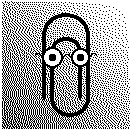
\includegraphics[height=10em]{assets/vigor.png}
			\caption{Vigor for VI}
			\label{figure:vigor}
		\end{figure}
	\end{minipage}
\end{center}

As we want \pcic sentences and not \gallina text, directly reading \coq vernac (.v) files will not be very useful.
During compilation of these vernac files \coq however generates \pcic terms internally.
These \pcic terms can be exported as so-called \acic terms using the \xml plugin distributed with \coq:
\begin{definition}[\acic]\defgls{acic}
	The Calculus of (Co)Inductive Constructions with Explicit Named Substitutions \cite{coen2000progettazione}.

	In normal \cic sections can contain local variables.
	After closing such a section, all definitions are discharged by abstracting these local section variables away.
	In \acic this is no longer necessary as the definitions are adapted to explicitly capture local variables.
\end{definition}

The tool is comprised of a \preloader and the main program \roerei.
The \preloader is implemented in \ocaml and handles importing the \xml generated by \coq and emitting summaries.
All other work, such as making predictions and measuring it's own performance is done by \roerei, which is implemented in \cpp.

The \machinelearning field favours \python and \matlab as the preferred development environments.
Thus we needed to re-implement various \machinelearning algorithms in \cpp.

\subsection{Transformations}
The premise selection tool works as follows, and can be summarised as in Figure \ref{figure:transformations}:
\begin{enumerate}
    \item Export all \coq objects from the standard library and the selected corpora to XML files during their compilation.
		\coq has an XML export functionality built in, until version 8.4pl5.
		Currently this is the only existing method to extract \coq objects.
		This process is more thoroughly described in Section \ref{section:extraction}.
	\item Read these objects from XML files back into canonical \acic\glsadd{acic} format in memory of the \preloader.
	\item From each \coqobj[s] of the form $\name[s] \objdef \term[s] : \type[s]$,
		yield a summary $<\name[s], \termset{s}, \typeset{s}>$.
		\begin{definition}[$\flatten{x}$]\defgls{flatten}
			For a given term (or type) $x$, yield the set of names referenced to in the term.
			\[ \flattensym : \terms \rightarrow 2^{\names} \]
		\end{definition}
		Given that definition, $\termset{s}$\glsadd{termset} is the set of names of all objects in the term $\term[s]$,
		and $\typeset{s}$\glsadd{typeset} is the set of all names in the type $\type[s]$.
		Note that other variants for this $\termset{s}$ can be used.
		In Section \ref{section:countoccur} we also extract the number of occurances of each name using $\countoccur{x}$\glsadd{countoccur}.
		Finally in Section \ref{section:depth} we extract the minimum depth each name occurs $\depth{x}$\glsadd{depth}.
		\begin{figure}[H]
			\[
				\begin{array}{rcl}
					\typeset{\texttt{O}}, \typeset{\texttt{S}}, \typeset{\texttt{nat\_id}}, \typeset{\texttt{plus}} & = & \{ \texttt{nat} \}\\
					\typeset{\texttt{nat\_ind}} & = & \{ 0, \texttt{S} \} \\
					\typeset{\texttt{plus\_0\_r}} & = & \{ \texttt{nat}, \texttt{eq}, \texttt{plus}, 0 \} \\
					& & \\
					\termset{\texttt{nat\_id}} & = & \emptyset \\
					\termset{\texttt{plus\_0\_r}} & = & \{ \texttt{eq\_sym}, \texttt{nat\_ind}, \texttt{eq\_refl}, \texttt{f\_equal}, \texttt{S} \}
				\end{array}
			\]
			\caption{Summaries yielded for the natural number example in Figure \ref{figure:natexample}}
		\end{figure}
		These summaries are written to disk, and read again into memory of \roerei.
	\item Distinguish theorems from other definitions, which yields the features and dependencies.
		Ideally we would like to take all objects of sort \sortprop to be the theorems.
		However this does not work in all cases, specifically for the \corn dataset.
		In order to solve this we use a heuristic as defined by Kaliszyk \cite{kaliszyk2014machine}.
		Where we consider $S$ to be the set of all \coq objects, we take
		\begin{definition}\defgls{defs}
			$\defs = \bigcup_{s \in S} \typeset{s}$
		\end{definition}
		\begin{definition}\defgls{thms}
			$\thms = (\bigcup_{s \in S} \termset{s}) \setminus \defs$
		\end{definition}
		This is more extensively explained in Section \ref{section:features}.
		\begin{figure}[H]
			\[
				\begin{array}{rcl}
					\defs & = & \{ 0, \texttt{S}, \texttt{nat}, \texttt{eq}, \texttt{plus} \} \\
					\thms & = & \{ \texttt{eq\_sym}, \texttt{nat\_ind}, \texttt{eq\_refl}, \texttt{f\_equal} \}
				\end{array}
			\]
			\caption{$\defs$ and $\thms$ for the natural number example in Figure \ref{figure:natexample}}
		\end{figure}
    \item From the $\thms$ and $\defs$ generate a \dagraph of dependencies and feature vector for all \coq objects.
		\todo{dagraph dependencies} \todo{feature vector}
	\item These features and dependencies can now be used to predict by bundling them with a predictor, for example \knn.
		\todo{predictors}
\end{enumerate}

\todo{crossvalidation}
\todo{metrics}
\todo{corpora}
\todo{combine predictors}
\todo{more features}

\begin{figure}[H]
	\centering
	\begin{tikzpicture}[auto, node distance=2.5cm, main/.style={draw,align=center}]
		\node[main] (coq) {\coqobj[s]\\inside coq};
		\node[main] (xml) [below of=coq] {XML\\representation};
		\node[main] (term) [below of=xml] {\coqobj[s]\\$\name \objdef \term : \type$};
		\node[main] (summary) [below of=term] {Summary\\$<\name[s], \termset{s}, \typeset{s}>$};
		\node[main] (definitions) [below right=2cm and 0cm of summary] {Definitions\\$\defs$};
		\node[main] (theorems) [below left=2cm and 0cm of summary] {Theorems\\$\thms$};
		\node[main] (features) [below of=definitions] {Features\\of theorems\\$\features$};
		\node[main] (dependencies) [below of=theorems] {Dependencies\\of theorems\\$\deps$};
		\node[main] (predictor) [below=7.0cm of summary] {Predictor};

		\draw[->] (coq) edge node {(1) Coq XML export} (xml);
		\draw[->] (xml) edge node {(2) Parser} (term);
		\draw[->] (term) edge node {(3) Resolver} (summary);
		\draw[->] (summary) edge node [right] {(4) $\bigcup_{s \in S} \typeset{s}$} (definitions);
		\draw[->] (summary) edge node [left] {$\bigcup_{s \in S} \termset{s} \setminus \defs$ (4)} (theorems);
		\draw[dashed] (definitions) edge node {(4)} (theorems);
		\draw[->] (theorems) edge node {(5)} (dependencies);
		\draw[->] (definitions) edge node {(5)} (features);
		\draw[->] (features) edge node [left] {(6)} (predictor);
		\draw[->] (dependencies) edge node [right] {(6)} (predictor);
	\end{tikzpicture}
	\caption{Transformations performed by the \premiseselection tooling.}
	\label{figure:transformations}
\end{figure}


\subsection{Extraction}
\label{section:extraction}
The \coq XML plugin exports various objects.
After parsing the XML output only some of these constructs are used.
Of these, the following \coq objects are used:
\begin{description}
    \item[(Co)Inductive definitions]
        \coq allows for (co)inductive definitions.
        These definitions are composed of a name, a type, and a list of constructors.
        Each constructor also is composed of a name and a type.
        A constructor is a valid definition which can be used in theorems.
		A (Co)Inductive definition also yields an induction principle (\texttt{ind}) and a recursion scheme (\texttt{rec}).
		These are also separately exported by \coq, and thus need not be considered further.

    \item[Constants (definitions / theorems / axioms)]
        The types and bodies of constants are defined separately, as needed.
        Theorems are proof-irrelevant, whilst definitions need to be substituted when applied.
        These objects they become undistinguishable when exported.
        Axioms only generate a type, and no body.
\end{description}

The following objects are not used, but could be useful in future work:
\begin{description}
    \item[Proof in progress]
        Consists of a name, a type, a body and a list of dependencies.
        These dependencies still need to be satisfied to complete the proof.
    \item[Tactics application]
        On a higher level, tactics can be applied in order to form a proof.
        These higher level constructs are dependant on the proof engine.
        A proof consisting of tactics can thus become invalid given another \coq version.
        For premise selection these tactics can help solve proofs more quickly, because the proofs they form are smaller.
\end{description}

\coq also exports variables, but these are not used.
A variable consists of a name and a type, and becomes a parameter when a theory which uses the variable is applied.
Thusfar there is no use for these variables within this project.

\subsection{Features and output}
\label{section:features}
When performing \premiseselection, only theorems are taken into account.
For other constants selecting premises is conceptually problematic.
As the training set, for each proven theorem the features are computed from the type of the corresponding \coqobj.
The definitions used in the term of a \coqobj are the desired result of the \premiseselection.
Hence, given the type of a new theorem to be proved, the \premiseselection yields a set of definitions which are likely to help prove the theorem.
These definitions are ordered by the probability the definition can be used in the proof.
This ordering is derived from the used definitions of similar complete theorems.
The similarity of complete theorems is captured in the model employed in the \premiseselection, and is derived from the features.

Distinguishing theorems from other definitions is not trivial.
Normally only definitions of kind \prop need to be considered as theorems.
However in the case of \corn the propositions are of type \cprop, which is of kind \kindtype.
Also the kind of a definition is not exported consistently by \coq \citationeeded.
Instead we will initially use a heuristic as defined by Kaliszyk \cite{kaliszyk2014machine}.
This heuristic defines the theorems, or the set of allowed dependencies, as all definitions except those used in the types of definitions.

For \roerei only the definitions used in the theorem type are regarded as features.
Concretely, for a set of proven theorems $S$ with their types and bodies, the used definitions from the types are collected.
From this for each proven theorem $s$ a function $\features[s]$ is defined on the set of allowed features $Z$.
$Z$ is composed of the definitions $\defs$ as well as various other metrics which have been added halfway through this thesis such as the number of conjunctions in the type of a term.
$$ Z = \defs \cup \{ \wedge \} $$
$$
\begin{array}{lcl}
	\features[s] & : & \featurekeys \rightarrow \mathbb{R} \\
	\features[s](x) & = & \left\{
		\begin{array}{ll}
			\counttype{s}{x} & x \in \defs \\
			\counttype{s}{\wedge} & x = \wedge
		\end{array} \right.
\end{array}
$$
For the body of each proven theorem the used definitions are similarly collected, and the set of allowed dependencies $\deps[s]$ is constructed.

\subsubsection{Number of occurances}
\label{section:countoccur}

\subsubsection{Depth}
\label{section:depth}

\subsection{Predictors}

\begin{definition}{Predictor}
	\[ P : \features[s] \rightarrow \deps \rightharpoondown \mathbb{R} \]
\end{definition}

A predictor $p$ can now, for a unproven conjecture $c$,
using the features of said conjecture $\features[c]$,
compute the partial ordered set of definitions likely to be useful in the yet to be constructed proof of $c$.
\todo{Now a partial function on $\mathbb{R}$, how to denote partial ordered set?}
Each of these suggestions has an associated likelyhood $r_p$ to be useful in the proof of conjecture $c$.

\subsubsection{\knn}
$$ \text{dist}(x, y) = \left( \sum_{i \in \featurekeys} \left( \features[x](i) - \features[y](i) \right)^2 \right)^{\frac{1}{2}} $$

For a conjecture $c$ the distance using $\text{dist}$ is computed with each term $t \in \objs$.
Then the closest $K$ terms are selected, which we call $\text{closest}_K(c)$.
Their dependencies $\phi \in \deps[t]$ are then suggested.
Their likelyhood is dependant on the distance of their parents to conjecture $c$.
\[ r_\text{knn}(\phi, c) = \sum_{t \in \text{closest}_K(c)} \countbody{t}{\phi} \times \text{dist}(c, t) \]

\subsubsection{\nb}

Given dependency candidate $\phi$, we compute for all features $x \in \featurekeys$:
\[
	w_x = \tau + \sum_{\psi \in \parents[\phi]} \features[\psi](x) ~~\text{with}~~ W = \tau + \sum_{x \in \featurekeys} w_x - \tau
\]

Now we can compute the likelyhood of candidate $\phi$ given some constants $\pi, \sigma, \tau$:
\[
	r_\text{nb}(\phi, c) = \ln W +
	\sum_{x \in \featurekeys | w_x = 0} \features[c](x) \times \sigma +
	\sum_{x \in \featurekeys | w_x \neq 0} \features[c](x) \times \ln(\pi \times w_x) - \ln(W)
\]

By K\"uhlwein \cite{kuhlwein2013mash} it is suggested to use $\pi = 10$, $\sigma = -15$ and $\tau = 20$.

\subsubsection{Kernel methods}
\subsubsection{Deep neural nets}
\subsubsection{Random forests}
\subsubsection{SInE}
\subsubsection{MePo}
\subsubsection{Ensembles}

\subsection{Example}

\begin{lstlisting}[language=Coq, mathescape, frame=none]
$\defs = \{$nat$,$ 0$,$ S$,$ plus$\}$
\end{lstlisting}

\begin{lstlisting}[language=Coq, mathescape, frame=none]
$\thms = \mathtt{dom}(S) \setminus \defs = \{$nat_ind$,$ plus_0_r$\}$
\end{lstlisting}

\subsection{Performance}
The performance of a predictor is estimated by running the prediction on known corpora.
The results of these predictions are quantified using a set of metrics.

In order to prevent so-called overfitting bias, \crossvalidation is used.

% Cross validation on Corpora
% `Proof in Progress` -> step (aconstr)
% Subset corpora (Train) -> Corpus (Test) -> Rating
% A corpus is divided into Proofs in Progress (each substep)
% Ratio of guessed steps

It is customary to implement cross validation for premise selection in the following manner:
Construct a poset of objects from $\objs$ using the dependency relation for $x, y \in \objs$:
\[
	x <_D y ~~\leftrightarrow~~ \depstrans[x] \cap (\parentstrans[y] \cup \{y\}) \neq \emptyset
\]

A linearized list is constructed from this poset, and each element in this list is first tested, i.e. treated as a conjecture.
The predictor is asked for a prediction, and the performance is measured.
Finally the element is learned to the predictor by adding it to the trainingset and adding it to the allowed set of dependencies.

Currently, the predictor is trained using the entire trainingset of the fold, without the dependencies of the term-turned-conjecture $\phi$:
\[
	\trainset' = \trainset \setminus \depstrans[\phi] ~\text{and}~ \deps' = \deps \setminus \depstrans[\phi]
\]

Using the customary approach, always an equal or better performance is reached.
Trivially this can be concluded because some of the irrelevant terms are excluded from the trainingset, as a result of the poset linearization.
\todo{Explain posetcons \{optimistic, pessimistic, canonical\}}

\subsection{Corpora}
A corpus can have different characteristics, which might reveal strengths or weaknesses of predictors.
The following corpora are used as test cases:

\begin{description}
	\item[\coq stdlib]
	\item[\compcert]
    \item[\formalin]
    \item[\corn]
    \item[\mathcomp]
\end{description}

\subsection{Metrics}
Given a predictor, the performance of this predictor can be denoted using various metrics.
In this thesis we use the following metrics:

\todo{Explain Top100, suggestions, required, etc}

\begin{definition}{100Cover}
The average coverage of the set of proof dependencies by the first 100 suggestions.

\[ \text{100Cover} = \frac{ \#( \text{Top}_{100}(\text{Suggestions}) \bigcap \text{Required}) } { \#\text{Required} } \]
\end{definition}


\begin{definition}{100Precision}
\[ \text{100Precision} = \frac{ \#( \text{Top}_{100}(\text{Suggestions}) \bigcap \text{Required}) } { \#\text{Top}_{100}(\text{Suggestions}) } \]
\end{definition}

\begin{definition}{Recall}
\end{definition}

\begin{definition}{Rank}
\end{definition}

\begin{definition}{Area Under Curve (AUC)}
\end{definition}

